% Author: Izaak Neutelings (Februari, 2020)
\documentclass[border=3pt,tikz]{standalone}
\usepackage{amssymb}
\usepackage{physics}
\usepackage{bm}
\usepackage{tikz}
\tikzset{>=latex} % for LaTeX arrow head
\usepackage{xcolor}
\colorlet{veccol}{orange!90!black}
\colorlet{myblue}{blue!60!black}
\tikzstyle{vector}=[->,thick,veccol]
\def\R{1.4}
\def\r{0.03}
\def\N{9}
%\bm{\odot}%otimes
\def\RC{0.14}
\def\Cout{
  \tikz[baseline=-2.5]{ \draw[line width=0.7,myblue] (0,0) circle (\RC);
                        \fill[myblue] (0,0) circle (0.028); }
}
\def\Cin{
  \tikz[baseline=-2.5]{ \draw[line width=0.7,myblue] (0,0) circle (\RC)
                                                     (-135:0.75*\RC) -- (45:0.75*\RC)
                                                     (135:0.75*\RC) -- (-45:0.75*\RC); }
}
\def\null{\color{myblue}{0}}

\begin{document}


% ZERO - solenoid
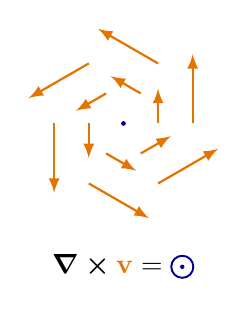
\begin{tikzpicture}
  \def\ang{60}
  \def\N{6}
  \fill[myblue] (0,0) circle (\r);
  %\foreach \x/\y in {-1/0,-1/1,0/1,1/1,1/0,-1/-1,0/-1,1/-1}{
  %  \draw[vector] (\x*0.5*\R,\y*0.5*\R) --++ (-\y*0.2*\R,\x*0.2*\R);
  %}
  \foreach \R in {0.44,0.88}{
    \foreach \i [evaluate={\ang=\i*360/\N;}] in {1,...,\N}{
      \draw[vector] (\ang:\R) --++ (\ang+90:\R);
    }
  }
  %\foreach \i [evaluate={\ang=\i*360/\N;}] in {1,...,\N}{
  %  \draw[vector] (\x*0.5*\R,\y*0.5*\R) ++ (\ang-180:\R/2) --++ (\ang:\R);
  %}
  \node at (0,-1.3*\R) {$\curl{{\color{veccol}\vb{v}}} = \Cout$};
\end{tikzpicture}


% RADIAL OUTWARD
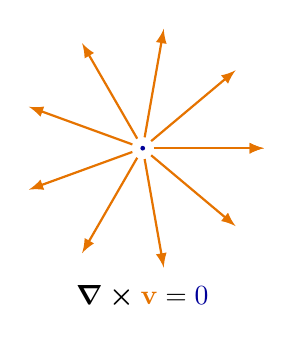
\begin{tikzpicture}
  \fill[myblue] (0,0) circle (\r);
  \foreach \i [evaluate={\ang=\i*360/\N;}] in {0,...,\N}{
    \draw[vector] (\ang:0.1*\R) --++ (\ang:\R);
  }
  \node at (0,-1.35*\R) {$\curl{{\color{veccol}\vb{v}}} = \null$};
\end{tikzpicture}


% RADIAL INWARD
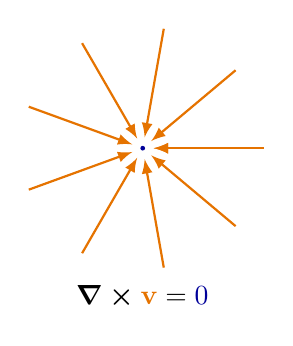
\begin{tikzpicture}
  \fill[myblue] (0,0) circle (\r);
  \foreach \i [evaluate={\ang=\i*360/\N;}] in {0,...,\N}{
    \draw[vector] (\ang:1.1*\R) -- (\ang:0.1*\R);
  }
  \node at (0,-1.35*\R) {$\curl{{\color{veccol}\vb{v}}} = \null$};
\end{tikzpicture}


% ZERO
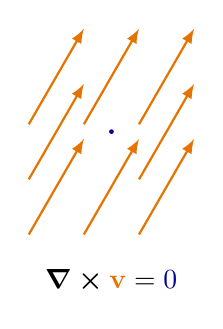
\begin{tikzpicture}
  \def\ang{60}
  \fill[myblue] (0,0) circle (\r);
  \foreach \x/\y in {-1/0,-1/1,0/1,1/1,1/0,-1/-1,0/-1,1/-1}{
    \draw[vector] (\x*0.5*\R,\y*0.5*\R) ++ (\ang-180:\R/2) --++ (\ang:\R);
  }
  \node at (0,-1.35*\R) {$\curl{{\color{veccol}\vb{v}}} = \null$};
\end{tikzpicture}


% ZERO
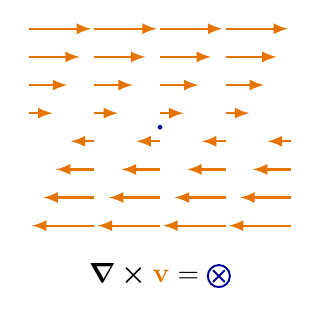
\begin{tikzpicture}
  \def\ang{60}
  \def\Ny{4}
  \def\Nx{4}
  \def\L{2.5}
  \fill[myblue] (0,0) circle (\r);
  \foreach \i [evaluate={\y=(\i-0.5)*(\L/2)/(\Ny-0.5); \r=0.3*\i^(0.7)}] in {1,...,\Ny}{
    \foreach \j [evaluate={\x=-\L/2+(\j-1.5)*\L/(\Nx-1);}] in {1,...,\Nx}{
      \draw[vector] ( \x, \y) --++ ( \r,0);
      \draw[vector] (-\x,-\y) --++ (-\r,0);
    }
  }
  \node at (0,-1.35*\R) {$\curl{{\color{veccol}\vb{v}}} = \Cin$};
\end{tikzpicture}


\end{document}
